% Options for packages loaded elsewhere
\PassOptionsToPackage{unicode}{hyperref}
\PassOptionsToPackage{hyphens}{url}
%
\documentclass[
]{article}
\usepackage{amsmath,amssymb}
\usepackage{iftex}
\ifPDFTeX
  \usepackage[T1]{fontenc}
  \usepackage[utf8]{inputenc}
  \usepackage{textcomp} % provide euro and other symbols
\else % if luatex or xetex
  \usepackage{unicode-math} % this also loads fontspec
  \defaultfontfeatures{Scale=MatchLowercase}
  \defaultfontfeatures[\rmfamily]{Ligatures=TeX,Scale=1}
\fi
\usepackage{lmodern}
\ifPDFTeX\else
  % xetex/luatex font selection
\fi
% Use upquote if available, for straight quotes in verbatim environments
\IfFileExists{upquote.sty}{\usepackage{upquote}}{}
\IfFileExists{microtype.sty}{% use microtype if available
  \usepackage[]{microtype}
  \UseMicrotypeSet[protrusion]{basicmath} % disable protrusion for tt fonts
}{}
\makeatletter
\@ifundefined{KOMAClassName}{% if non-KOMA class
  \IfFileExists{parskip.sty}{%
    \usepackage{parskip}
  }{% else
    \setlength{\parindent}{0pt}
    \setlength{\parskip}{6pt plus 2pt minus 1pt}}
}{% if KOMA class
  \KOMAoptions{parskip=half}}
\makeatother
\usepackage{xcolor}
\usepackage{color}
\usepackage{fancyvrb}
\newcommand{\VerbBar}{|}
\newcommand{\VERB}{\Verb[commandchars=\\\{\}]}
\DefineVerbatimEnvironment{Highlighting}{Verbatim}{commandchars=\\\{\}}
% Add ',fontsize=\small' for more characters per line
\newenvironment{Shaded}{}{}
\newcommand{\AlertTok}[1]{\textcolor[rgb]{1.00,0.00,0.00}{\textbf{#1}}}
\newcommand{\AnnotationTok}[1]{\textcolor[rgb]{0.38,0.63,0.69}{\textbf{\textit{#1}}}}
\newcommand{\AttributeTok}[1]{\textcolor[rgb]{0.49,0.56,0.16}{#1}}
\newcommand{\BaseNTok}[1]{\textcolor[rgb]{0.25,0.63,0.44}{#1}}
\newcommand{\BuiltInTok}[1]{\textcolor[rgb]{0.00,0.50,0.00}{#1}}
\newcommand{\CharTok}[1]{\textcolor[rgb]{0.25,0.44,0.63}{#1}}
\newcommand{\CommentTok}[1]{\textcolor[rgb]{0.38,0.63,0.69}{\textit{#1}}}
\newcommand{\CommentVarTok}[1]{\textcolor[rgb]{0.38,0.63,0.69}{\textbf{\textit{#1}}}}
\newcommand{\ConstantTok}[1]{\textcolor[rgb]{0.53,0.00,0.00}{#1}}
\newcommand{\ControlFlowTok}[1]{\textcolor[rgb]{0.00,0.44,0.13}{\textbf{#1}}}
\newcommand{\DataTypeTok}[1]{\textcolor[rgb]{0.56,0.13,0.00}{#1}}
\newcommand{\DecValTok}[1]{\textcolor[rgb]{0.25,0.63,0.44}{#1}}
\newcommand{\DocumentationTok}[1]{\textcolor[rgb]{0.73,0.13,0.13}{\textit{#1}}}
\newcommand{\ErrorTok}[1]{\textcolor[rgb]{1.00,0.00,0.00}{\textbf{#1}}}
\newcommand{\ExtensionTok}[1]{#1}
\newcommand{\FloatTok}[1]{\textcolor[rgb]{0.25,0.63,0.44}{#1}}
\newcommand{\FunctionTok}[1]{\textcolor[rgb]{0.02,0.16,0.49}{#1}}
\newcommand{\ImportTok}[1]{\textcolor[rgb]{0.00,0.50,0.00}{\textbf{#1}}}
\newcommand{\InformationTok}[1]{\textcolor[rgb]{0.38,0.63,0.69}{\textbf{\textit{#1}}}}
\newcommand{\KeywordTok}[1]{\textcolor[rgb]{0.00,0.44,0.13}{\textbf{#1}}}
\newcommand{\NormalTok}[1]{#1}
\newcommand{\OperatorTok}[1]{\textcolor[rgb]{0.40,0.40,0.40}{#1}}
\newcommand{\OtherTok}[1]{\textcolor[rgb]{0.00,0.44,0.13}{#1}}
\newcommand{\PreprocessorTok}[1]{\textcolor[rgb]{0.74,0.48,0.00}{#1}}
\newcommand{\RegionMarkerTok}[1]{#1}
\newcommand{\SpecialCharTok}[1]{\textcolor[rgb]{0.25,0.44,0.63}{#1}}
\newcommand{\SpecialStringTok}[1]{\textcolor[rgb]{0.73,0.40,0.53}{#1}}
\newcommand{\StringTok}[1]{\textcolor[rgb]{0.25,0.44,0.63}{#1}}
\newcommand{\VariableTok}[1]{\textcolor[rgb]{0.10,0.09,0.49}{#1}}
\newcommand{\VerbatimStringTok}[1]{\textcolor[rgb]{0.25,0.44,0.63}{#1}}
\newcommand{\WarningTok}[1]{\textcolor[rgb]{0.38,0.63,0.69}{\textbf{\textit{#1}}}}
\usepackage{graphicx}
\makeatletter
\def\maxwidth{\ifdim\Gin@nat@width>\linewidth\linewidth\else\Gin@nat@width\fi}
\def\maxheight{\ifdim\Gin@nat@height>\textheight\textheight\else\Gin@nat@height\fi}
\makeatother
% Scale images if necessary, so that they will not overflow the page
% margins by default, and it is still possible to overwrite the defaults
% using explicit options in \includegraphics[width, height, ...]{}
\setkeys{Gin}{width=\maxwidth,height=\maxheight,keepaspectratio}
% Set default figure placement to htbp
\makeatletter
\def\fps@figure{htbp}
\makeatother
\setlength{\emergencystretch}{3em} % prevent overfull lines
\providecommand{\tightlist}{%
  \setlength{\itemsep}{0pt}\setlength{\parskip}{0pt}}
\setcounter{secnumdepth}{-\maxdimen} % remove section numbering
\ifLuaTeX
  \usepackage{selnolig}  % disable illegal ligatures
\fi
\IfFileExists{bookmark.sty}{\usepackage{bookmark}}{\usepackage{hyperref}}
\IfFileExists{xurl.sty}{\usepackage{xurl}}{} % add URL line breaks if available
\urlstyle{same}
\hypersetup{
  hidelinks,
  pdfcreator={LaTeX via pandoc}}

\author{}
\date{}

\begin{document}

\hypertarget{ux5b9eux9a8cux56db}{%
\section{实验四}\label{ux5b9eux9a8cux56db}}

\hypertarget{ux4e00ux95eeux9898ux5206ux6790}{%
\subsection{一、问题分析}\label{ux4e00ux95eeux9898ux5206ux6790}}

\hypertarget{ux95eeux9898ux4e0eux529fux80fdux63cfux8ff0}{%
\subsubsection{问题与功能描述:}\label{ux95eeux9898ux4e0eux529fux80fdux63cfux8ff0}}

【问题描述】

二叉树的合并

给定两个二叉树,将它们中的一个覆盖到另一个上时,两个二叉树的一些节点便会重叠,你需要根据规则将他们合并为一个新的二叉树。合并的规则是如果两个节点重叠,那么将它们的值相加作为节点合并后的新值,否则不为
NULL 的节点将直接作为新二叉树的节点。

示例 :

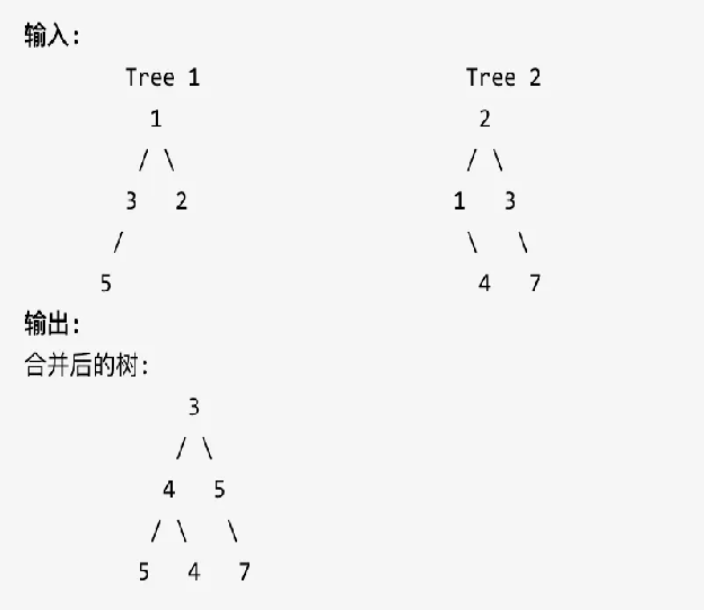
\includegraphics{E:/Desktop/学习/数据结构/实验/实验四/实验二.assets/image-20230412154039745.png}

【输入形式】

每个输入文件的第一行为二叉树A的前序遍历顺序表示法(N≤30)。

第二行为二叉树B的前序遍历顺序表示法(N≤30)。

注意:用``\#''代表空指针NULL。

【输出形式】

输出为合并之后的二叉树的前序遍历顺序表示法。用``\#''代表空指针NULL。

\hypertarget{ux6837ux4f8bux5206ux6790}{%
\subsubsection{样例分析:}\label{ux6837ux4f8bux5206ux6790}}

求解方法:题目要求合并两个二叉树,如果对应节点有重叠,则将它们的值相加作为合并后的节点的新值;否则,不为NULL的节点将直接作为新二叉树的节点。

因此,我们可以按照以下步骤来实现合并:

\begin{enumerate}
\def\labelenumi{\arabic{enumi}.}
\item
  对于两个给定的二叉树,分别遍历它们,得到它们的前序遍历序列。
\item
  从两个序列的第一个节点开始比较,如果它们都不为NULL,则将它们的值相加,并新建一个节点存储相加后的值。
\item
  如果其中一个节点为NULL,则将另一个节点作为新建节点的左或右孩子节点。
\item
  对新建节点的左右孩子节点递归执行上述合并操作,直到两个序列中的所有节点都被处理完毕。
\item
  最后,得到的二叉树即为合并后的结果。
\end{enumerate}

需要注意的是,在合并两个节点的值时,需要考虑两个节点都为NULL的情况,此时新建一个节点存储0值。此外,由于题目中规定了节点值不会超过9,因此可以将节点值转化为字符型处理,而不是直接存储为整型。

【样例输入1】

135\#\#\#2\#\#

21\#4\#\#3\#7\#\#

【样例输出1】

345\#\#4\#\#5\#7\#\#

【样例输入2】

324\#\#3\#\#235\#\#\#5\#\#

323\#\#\#\#

【样例输出2】

647\#\#3\#\#235\#\#\#5\#\#

【样例输入3】

324\#\#3\#\#235\#\#\#5\#\#

232\#\#\#5\#\#

【样例输出3】

556\#\#3\#\#735\#\#\#5\#\#

\hypertarget{ux6570ux636eux7ed3ux6784ux5206ux6790}{%
\subsubsection{数据结构分析:}\label{ux6570ux636eux7ed3ux6784ux5206ux6790}}

【抽象数据类型设计】

二叉树 BinNode:

\begin{itemize}
\item
  数据成员:

  \begin{itemize}
  \item
    value:节点的值
  \item
    left:节点的左子树
  \item
    right:节点的右子树
  \end{itemize}
\item
  成员函数:

  \begin{itemize}
  \item
    getValue():获取节点的值
  \item
    setValue():设置节点的值
  \item
    left():获取节点的左子树
  \item
    setLeft():设置节点的左子树
  \item
    right():获取节点的右子树
  \item
    setRight():设置节点的右子树
  \end{itemize}
\end{itemize}

【物理数据对象设计】

采用二叉链表存储结构实现二叉树 BinNode。

具体实现可参考 tree.h 和 TTree.h 文件中的代码。

【算法思想的设计】

二叉树的递归遍历。

【关键功能的算法步骤】

\begin{enumerate}
\def\labelenumi{\arabic{enumi}.}
\item
  读入两个二叉树的前序遍历顺序表示法,创建二叉树 BinNode1 和 BinNode2。
\item
  定义递归函数 mergeTrees,将二叉树 BinNode1 和 BinNode2
  合并成一个新的二叉树。
\item
  若其中一个节点为空,则直接返回另一个节点。
\item
  新建一个节点 tmp,节点值为两个节点的值相加。
\item
  将两个节点的左子树递归合并,将结果设置为 tmp 的左子树。
\item
  将两个节点的右子树递归合并,将结果设置为 tmp 的右子树。
\item
  返回 tmp。
\item
  调用 mergeTrees 函数得到合并后的二叉树 BinNode3。
\item
  对合并后的二叉树进行前序遍历输出。
\end{enumerate}

注:节点值为字符,需要将其转换为数字类型。

【物理实现】

\begin{Shaded}
\begin{Highlighting}[]
\NormalTok{BinNode}\OperatorTok{\textless{}}\DataTypeTok{int}\OperatorTok{\textgreater{}} \OperatorTok{*}\NormalTok{creatBinaryTree}\OperatorTok{()} \OperatorTok{\{}

	\DataTypeTok{char}\NormalTok{ c}\OperatorTok{;}

\NormalTok{	cin }\OperatorTok{\textgreater{}\textgreater{}}\NormalTok{ c}\OperatorTok{;}

	\ControlFlowTok{if} \OperatorTok{(}\NormalTok{c }\OperatorTok{==} \CharTok{\textquotesingle{}\#\textquotesingle{}}\OperatorTok{)}

		\ControlFlowTok{return}\NormalTok{ NULL}\OperatorTok{;}

\NormalTok{	BinNode}\OperatorTok{\textless{}}\DataTypeTok{int}\OperatorTok{\textgreater{}} \OperatorTok{*}\NormalTok{root }\OperatorTok{=} \KeywordTok{new}\NormalTok{ BinNode}\OperatorTok{\textless{}}\DataTypeTok{int}\OperatorTok{\textgreater{};}

\NormalTok{	root}\OperatorTok{{-}\textgreater{}}\NormalTok{setValue}\OperatorTok{((}\DataTypeTok{int}\OperatorTok{)}\NormalTok{c }\OperatorTok{{-}} \DecValTok{48}\OperatorTok{);}

\NormalTok{	root}\OperatorTok{{-}\textgreater{}}\NormalTok{setLeft}\OperatorTok{(}\NormalTok{creatBinaryTree}\OperatorTok{());}

\NormalTok{	root}\OperatorTok{{-}\textgreater{}}\NormalTok{setRight}\OperatorTok{(}\NormalTok{creatBinaryTree}\OperatorTok{());}

	\ControlFlowTok{return}\NormalTok{ root}\OperatorTok{;}

\OperatorTok{\}}



\NormalTok{BinNode}\OperatorTok{\textless{}}\DataTypeTok{int}\OperatorTok{\textgreater{}} \OperatorTok{*}\NormalTok{mergeTrees}\OperatorTok{(}\NormalTok{BinNode}\OperatorTok{\textless{}}\DataTypeTok{int}\OperatorTok{\textgreater{}} \OperatorTok{*}\NormalTok{t1}\OperatorTok{,}\NormalTok{ BinNode}\OperatorTok{\textless{}}\DataTypeTok{int}\OperatorTok{\textgreater{}} \OperatorTok{*}\NormalTok{t2}\OperatorTok{)} \OperatorTok{\{}

	\ControlFlowTok{if} \OperatorTok{(}\NormalTok{t2 }\OperatorTok{==}\NormalTok{ NULL}\OperatorTok{)}

		\ControlFlowTok{return}\NormalTok{ t1}\OperatorTok{;}

	\ControlFlowTok{if} \OperatorTok{(}\NormalTok{t1 }\OperatorTok{==}\NormalTok{ NULL}\OperatorTok{)}

		\ControlFlowTok{return}\NormalTok{ t2}\OperatorTok{;}

\NormalTok{	BinNode}\OperatorTok{\textless{}}\DataTypeTok{int}\OperatorTok{\textgreater{}} \OperatorTok{*}\NormalTok{tmp }\OperatorTok{=} \KeywordTok{new}\NormalTok{ BinNode}\OperatorTok{\textless{}}\DataTypeTok{int}\OperatorTok{\textgreater{};}

\NormalTok{	tmp}\OperatorTok{{-}\textgreater{}}\NormalTok{setValue}\OperatorTok{(}\NormalTok{t1}\OperatorTok{{-}\textgreater{}}\NormalTok{getValue}\OperatorTok{()} \OperatorTok{+}\NormalTok{ t2}\OperatorTok{{-}\textgreater{}}\NormalTok{getValue}\OperatorTok{());}

\NormalTok{	tmp}\OperatorTok{{-}\textgreater{}}\NormalTok{setLeft}\OperatorTok{(}\NormalTok{mergeTrees}\OperatorTok{(}\NormalTok{t1}\OperatorTok{{-}\textgreater{}}\NormalTok{left}\OperatorTok{(),}\NormalTok{ t2}\OperatorTok{{-}\textgreater{}}\NormalTok{left}\OperatorTok{()));}

\NormalTok{	tmp}\OperatorTok{{-}\textgreater{}}\NormalTok{setRight}\OperatorTok{(}\NormalTok{mergeTrees}\OperatorTok{(}\NormalTok{t1}\OperatorTok{{-}\textgreater{}}\NormalTok{right}\OperatorTok{(),}\NormalTok{ t2}\OperatorTok{{-}\textgreater{}}\NormalTok{right}\OperatorTok{()));}

	\ControlFlowTok{return}\NormalTok{ tmp}\OperatorTok{;}

\OperatorTok{\}}



\DataTypeTok{void}\NormalTok{ printNode}\OperatorTok{(}\NormalTok{BinNode}\OperatorTok{\textless{}}\DataTypeTok{int}\OperatorTok{\textgreater{}} \OperatorTok{*}\NormalTok{root}\OperatorTok{)} \OperatorTok{\{}

	\ControlFlowTok{if} \OperatorTok{(}\NormalTok{root}\OperatorTok{)} \OperatorTok{\{}

\NormalTok{		cout }\OperatorTok{\textless{}\textless{}}\NormalTok{ root}\OperatorTok{{-}\textgreater{}}\NormalTok{getValue}\OperatorTok{();}

\NormalTok{		printNode}\OperatorTok{(}\NormalTok{root}\OperatorTok{{-}\textgreater{}}\NormalTok{left}\OperatorTok{());}

\NormalTok{		printNode}\OperatorTok{(}\NormalTok{root}\OperatorTok{{-}\textgreater{}}\NormalTok{right}\OperatorTok{());}

	\OperatorTok{\}}\NormalTok{ else
}
\NormalTok{		printf}\OperatorTok{(}\StringTok{"\#"}\OperatorTok{);}

\OperatorTok{\}}
\end{Highlighting}
\end{Shaded}

代码分析过程如下:

\begin{enumerate}
\def\labelenumi{\arabic{enumi}.}
\item
  定义一个函数\texttt{creatBinaryTree()},用于根据前序遍历顺序表示法输入二叉树并构建相应的二叉树,返回二叉树的根节点。
\item
  定义一个函数\texttt{mergeTrees(BinNode\textless{}int\textgreater{}\ *t1,\ BinNode\textless{}int\textgreater{}\ *t2)},用于合并两棵二叉树\texttt{t1}和\texttt{t2},返回合并后的二叉树的根节点。
\item
  如果\texttt{t2}为NULL,则直接返回\texttt{t1}。
\item
  如果\texttt{t1}为NULL,则直接返回\texttt{t2}。
\item
  否则,定义一个新节点\texttt{tmp},该节点的值为\texttt{t1}和\texttt{t2}节点值之和。
\item
  \texttt{tmp}的左子树为合并\texttt{t1}的左子树和\texttt{t2}的左子树,即\texttt{mergeTrees(t1-\textgreater{}left(),\ t2-\textgreater{}left())}。
\item
  \texttt{tmp}的右子树为合并\texttt{t1}的右子树和\texttt{t2}的右子树,即\texttt{mergeTrees(t1-\textgreater{}right(),\ t2-\textgreater{}right())}。
\item
  返回\texttt{tmp}。
\item
  定义一个函数\texttt{printNode(BinNode\textless{}int\textgreater{}\ *root)},用于前序遍历输出二叉树。
\item
  在\texttt{main()}函数中,调用\texttt{creatBinaryTree()}函数构建两棵二叉树\texttt{root1}和\texttt{root2}。
\item
  调用\texttt{mergeTrees()}函数合并\texttt{root1}和\texttt{root2},得到合并后的二叉树的根节点。
\item
  调用\texttt{printNode()}函数前序遍历输出合并后的二叉树。
\end{enumerate}

\hypertarget{ux7b97ux6cd5ux5206ux6790}{%
\subsubsection{算法分析}\label{ux7b97ux6cd5ux5206ux6790}}

\hypertarget{ux5173ux952eux6b65ux9aa4}{%
\paragraph{关键步骤}\label{ux5173ux952eux6b65ux9aa4}}

\begin{Shaded}
\begin{Highlighting}[]
\DataTypeTok{int}\NormalTok{ main}\OperatorTok{()} \OperatorTok{\{}



\NormalTok{	BinNode}\OperatorTok{\textless{}}\DataTypeTok{int}\OperatorTok{\textgreater{}} \OperatorTok{*}\NormalTok{root1}\OperatorTok{,} \OperatorTok{*}\NormalTok{ root2}\OperatorTok{;}

\NormalTok{	root1 }\OperatorTok{=} \KeywordTok{new}\NormalTok{ BinNode}\OperatorTok{\textless{}}\DataTypeTok{int}\OperatorTok{\textgreater{};}

\NormalTok{	root2 }\OperatorTok{=} \KeywordTok{new}\NormalTok{ BinNode}\OperatorTok{\textless{}}\DataTypeTok{int}\OperatorTok{\textgreater{};}

\NormalTok{	root1 }\OperatorTok{=}\NormalTok{ creatBinaryTree}\OperatorTok{();}

\NormalTok{	root2 }\OperatorTok{=}\NormalTok{ creatBinaryTree}\OperatorTok{();}

\NormalTok{	BinNode}\OperatorTok{\textless{}}\DataTypeTok{int}\OperatorTok{\textgreater{}} \OperatorTok{*}\NormalTok{ans }\OperatorTok{=}\NormalTok{ mergeTrees}\OperatorTok{(}\NormalTok{root1}\OperatorTok{,}\NormalTok{ root2}\OperatorTok{);}

\NormalTok{	printNode}\OperatorTok{(}\NormalTok{ans}\OperatorTok{);}

	\ControlFlowTok{return} \DecValTok{0}\OperatorTok{;}

\OperatorTok{\}}
\end{Highlighting}
\end{Shaded}

\hypertarget{ux7b97ux6cd5ux6027ux80fdux5206ux6790}{%
\paragraph{算法性能分析}\label{ux7b97ux6cd5ux6027ux80fdux5206ux6790}}

该算法的时间复杂度取决于遍历二叉树的次数,即所有节点的数量,所以为O(n),其中n为所有节点的数量。

空间复杂度也取决于节点数量,每个节点需要一个存储该节点值的变量,以及指向左右子树的指针,所以空间复杂度也为O(n)。

综上,该算法的时间复杂度和空间复杂度都为O(n),其中n为所有节点的数量。

\end{document}
